\documentclass[conference]{IEEEtran}

% ---- Packages ----
\usepackage[utf8]{inputenc}       % UTF-8 encoding
\usepackage{cite}                 % Sorted & compressed numeric citations [1]-[3]
\usepackage{amsmath}              % Math environments
\usepackage{graphicx}             % Include images: \includegraphics{}
\usepackage{url}                  % Line-breakable URLs
\usepackage{lipsum}               % Lorem Ipsum text generation
\usepackage[colorlinks=true,
            allcolors=black]{hyperref}  % Clickable links, but black text
\usepackage{graphicx}
\usepackage{caption}
\usepackage{subcaption}
% ---- Title & Authors ----
\title{Your Generic Paper Title}

\author{\IEEEauthorblockN{Baoyi Liu, Cindy Lin, Guanghua Liu, Jiale Liu, Mingyuan Shao, Wenjie Ding, Zhuolun Li}
\IEEEauthorblockA{School of Computing, Newcastle University, Newcastle upon Tyne, United Kingdom \\
Email: \{11111111, 2222222, 33333333, 44444444, 5555555, 6666666, 7777777\}@newcastle.ac.uk}}

% ==================================================================
\begin{document}
\maketitle

% ---- Abstract ----
\begin{abstract}
  Write your abstract here. It should briefly state the problem,
  the approach, key results, and the conclusion (typically 150--250 words).
\end{abstract}

% ---- Keywords (optional) ----
\begin{IEEEkeywords}
  keyword one, keyword two, keyword three
\end{IEEEkeywords}

% ==================================================================
% SECTIONS — each teammate can edit their own section
% ==================================================================

\section{Introduction}
\label{sec:intro}
Rainfall prediction has become increasingly important for urban resilience and smart water management systems, particularly with the proliferation of IoT sensors and distributed environmental monitoring. While recent studies have achieved notable improvements in predictive modelling accuracy, many of them overlook system-level constraints such as communication cost, scalability, and deployment feasibility in resource-constrained environments (Chan et al., 2023; Elhindi et al., 2024). This limitation becomes more critical when rainfall forecasting models are deployed across edge devices connected via wireless networks. 

Federated Split Learning (FSL) has been proposed to reduce computational burden on edge devices by splitting model training between clients and a central server. By allowing early layers to be trained locally and later layers centrally, FSL reduces client-side computation while preserving data privacy. However, communication cost and scalability remain significant challenges. Frequent transmission of smashed activations and gradients leads to high communication overhead, and maintaining server-side states for multiple clients may limit scalability. Recent works attempt to mitigate these issues through dynamic split points, gradient aggregation, asynchronous training, or selective communication strategies (Mahmoudi et al., 2024; Ghadikolaei et al., 2024; Zhu et al., 2024). While these methods improve efficiency under certain conditions, they often increase architectural complexity, rely on centralized coordination, or assume relatively stable network conditions, limiting their adaptability in dynamic wireless environments. 

A related research direction focuses on communication-efficient federated learning through parameter compression. For example, compressive sensing–based approaches reduce bidirectional communication via adaptive compression ratios (Hafnavi et al., 2024). Similarly, communication-efficient personalized federated edge learning frameworks employ gradient compression to mitigate bandwidth pressure in wireless scenarios (Elhindi et al., 2024). These approaches effectively reduce the size of transmitted model updates. However, their optimization primarily targets gradients or weights in standard FL architectures. In Split FL settings, smashed activations transmitted between client and server can dominate communication overhead. Moreover, compression methods often rely on sparsity assumptions that may deteriorate as training progresses, potentially degrading reconstruction quality and model performance. Importantly, although transmission size is reduced, synchronization frequency is typically unchanged, meaning that communication events remain frequent. 

Other works attempt to reduce computation or storage overhead through model pruning and lightweight architectures. Adaptive pruning strategies adjust model complexity based on heterogeneous device capabilities, improving feasibility in resource-constrained environments (Zhu et al., 2024). Lightweight rainfall prediction models also aim to balance forecasting accuracy and computational efficiency (Elhindi et al., 2024). Nevertheless, these improvements remain largely structural. Clients usually continue to participate in each synchronization round, leaving the temporal communication pattern intact. As a result, cumulative communication cost may still be substantial even if model size is reduced. 

Across these categories, a consistent limitation emerges. Communication efficiency is typically addressed at a single layer—parameter compression (Hafnavi et al., 2024), model pruning (Zhu et al., 2024), architectural redesign in split learning (Mahmoudi et al., 2024; Ghadikolaei et al., 2024), or application-specific lightweight modelling (Chan et al., 2023; Elhindi et al., 2024). However, few studies systematically analyze communication behaviour within the Split FL interaction loop itself. In practical deployments, smashed activations may constitute a substantial portion of transmitted data, and synchronization frequency directly influences both bandwidth consumption and convergence stability. Yet the joint impact of activation representation and synchronization interval on communication–convergence trade-offs remains insufficiently quantified. 

This gap suggests that beyond structural or architectural modifications, there is a need to examine lightweight and adaptive mechanisms that directly control (i) how activations are represented during transmission and (ii) how often synchronization occurs between client and server. A systematic evaluation of these two factors under heterogeneous wireless conditions can provide clearer insight into the trade-offs between communication cost, accuracy degradation, and convergence behaviour, thereby informing more scalable and practical Split Federated Learning systems. 


\section{Related Work}
\label{sec:related}
% Survey existing literature and position your work.
\lipsum[3]
Recent work~\cite{ref3} shows that...
\lipsum[4]

\section{Methodology}
\label{sec:method}


\begin{figure*}[t]
    \centering
    % 第一张图：Architecture
    \begin{subfigure}{\textwidth} % 宽度设为 \textwidth 就会占据整行，自动换行
        \centering
        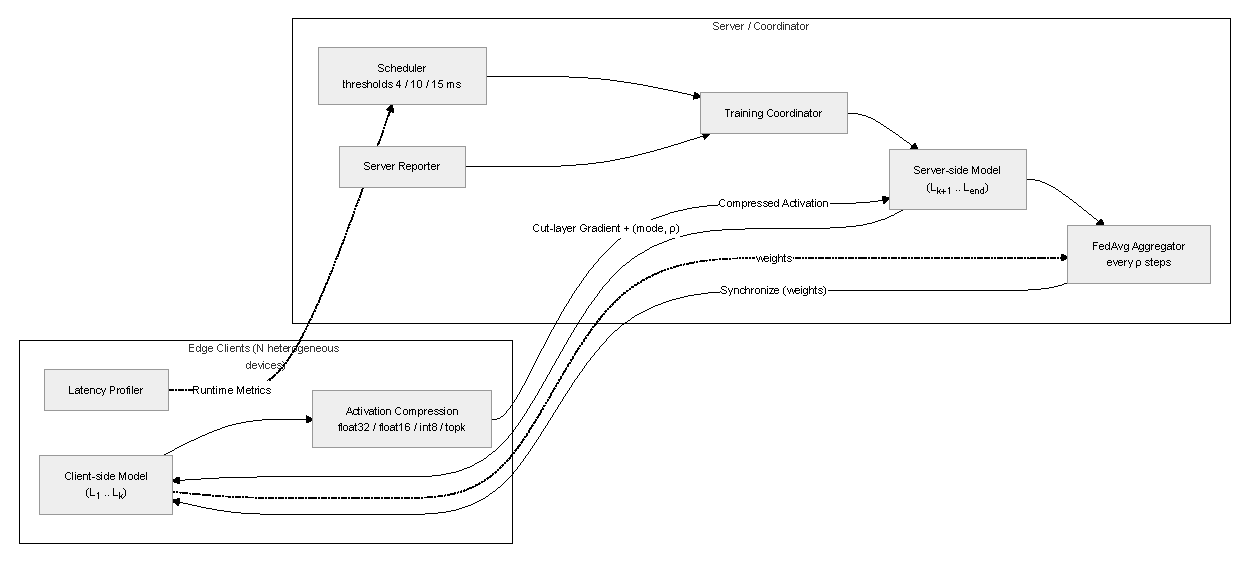
\includegraphics[width=0.9\textwidth]{diagrams/Architecture.pdf} % 这里的 0.8 是控制单张图的缩放
        \caption{System Architecture}
        \label{fig:arch}
    \end{subfigure}

    % 第二张图：Sequence
    \begin{subfigure}{\textwidth}
        \centering
        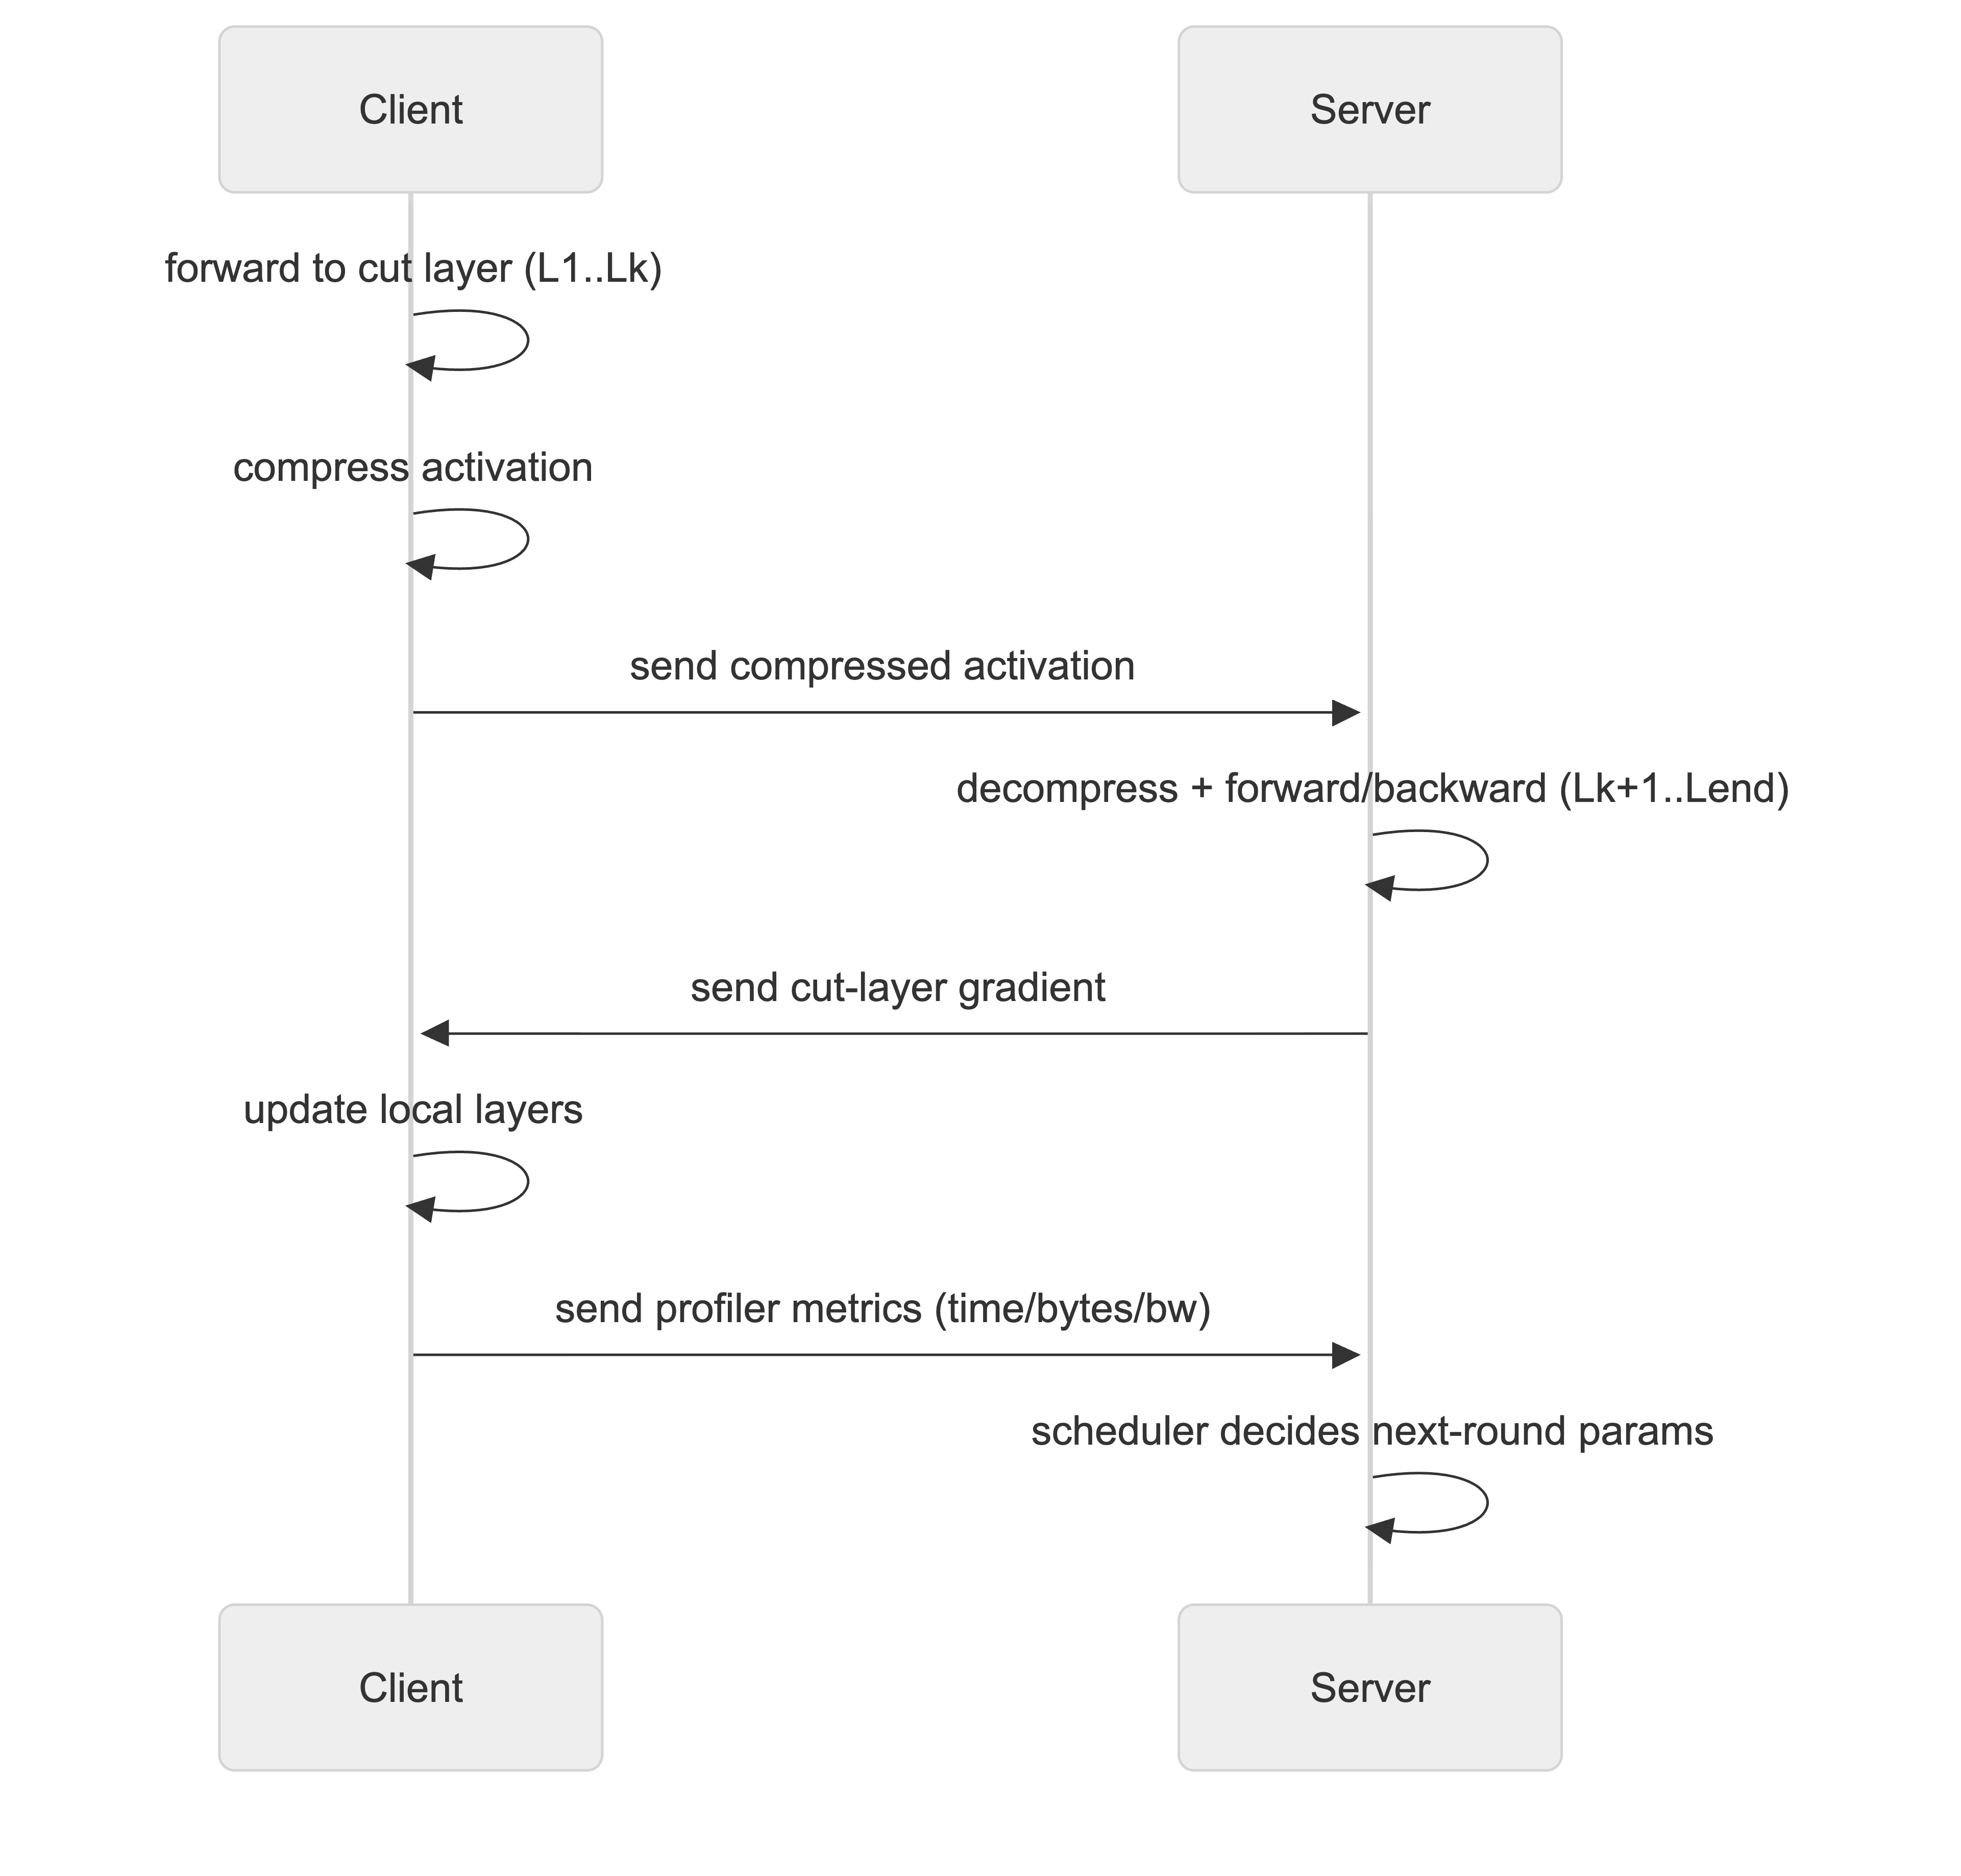
\includegraphics[width=0.9\textwidth]{diagrams/Sequence.pdf}
        \caption{Operation Sequence}
        \label{fig:seq}
    \end{subfigure}
    
    \caption{System design details: (a) physical architecture and (b) interaction sequence diagram.}
    \label{fig:full_design}
\end{figure*}


% ---- References ----
% Compile order: pdflatex -> bibtex -> pdflatex -> pdflatex
\bibliographystyle{IEEEtran}
\bibliography{IEEEabrv,refs}

\end{document}
